 % LuaLaTeX文書; 文字コーAドはUTF-8
 \documentclass[unicode,12pt, A4j]{ltjsarticle}% 'unicode'が必要
 %\usepackage{luatexja}% 日本語したい
 \usepackage{luatexja-fontspec}
 %\usepackage[hiragino-pron]{luatexja-preset}% IPAexフォントしたい(ipaex)
 \usepackage[hiragino-pron,deluxe,expert,bold]{luatexja-preset}

 \usepackage[english]{babel}%多言語文書を作成する
 \usepackage{amsmath,amssymb}%標準数式表現を拡大する
 \usepackage{physics}
 \usepackage[subpreambles=true,sort=true]{standalone}
% \renewcommand{\kanjifamilydefault}{\gtdefault}% 既定をゴシック体に
 \usepackage[backend=bibtex,style=phys,articletitle=false,biblabel=brackets,chaptertitle=false,pageranges=false]{biblatex}
 %\usepackage[style=authoryear,backend=bibtex]{biblatex}


 %\addbibresource{../references/tio2_ref.bib}
 \usepackage{mhchem}
 % あとは欧文の場合と同じ
  \usepackage{graphics}
  \usepackage{caption}
  \usepackage[subrefformat=parens]{subcaption}
\title{東大数学理科後期1991年度}
\author{}
\date{}

\begin{document}
\maketitle

\section{問題1}
\begin{enumerate}
 \item $x>0$において,関数$\log x/x$の増減を調べよ.ただし,$\log x$は$x$の自然対数である.
 \item 正整数$a$,$b$の組で,$a^b=b^a$かつ$a\neq b$を満たすものをすべて求めよ.
 \item $3^x=x^3$を満たす正の有理数は,$3$以外には存在しないことを示せ.
\end{enumerate}

\section{問題2}
平面上に$3$つの円$\mathrm{C}_1$,$\mathrm{C}_2$,$\mathrm{C}_3$があって,$\mathrm{C}_1$と$mathrm{C}_2$は相異なる$2$点$\mathrm{A}$,$\mathrm{B}$で交わり,$\mathrm{C}_3$は$\mathrm{C}_1$および$\mathrm{C}_2$と互いに直交している.ただし,$2$つの円が互いに直交しているとは,二つの円に共通点があって,各共通点におけるそれぞれの円に対する接線がその共通点で直交しているときをいう.
\begin{enumerate}
 \item 円$\mathrm{C}_3$の中身は,$2$点$\mathrm{A}$,$\mathrm{B}$を通る直線上にあることを示せ.
 \item $2$点$\mathrm{A}$,$\mathrm{B}$の一方は円$\mathrm{C}_3$の内側に,他方は円$\mathrm{C}_3$の外側にあることを示せ.
\end{enumerate}


\section{問題3}
$xy$平面上の長さ$2$の線分$\mathrm{AB}$を直径とする半円を$\mathrm{D}$とする.半円$\mathrm{D}$の内部(周を含まない)の一点を$\mathrm{P}$とする.$\mathrm{A}$と$\mathrm{P}$を通る直線と半円$\mathrm{D}$の円孤の部分との交点を$\mathrm{Q}$とし,$mathrm{B}$と$\mathrm{P}$を通る直線と半円$\mathrm{D}$の円弧の部分との交点を$\mathrm{R}$とする.五角形$\mathrm{ARPQB}$の面積を$S$とおく.
\begin{enumerate}
 \item $\angle \mathrm{APB}$を一定に保ったまま点$\mathrm{P}$が半円$\mathrm{D}$の内部を動くとき,$S$のとる値の範囲を$\angle APB=\theta$を使ってあらわせ.
 \item 点$\mathrm{P}$が,半円$\mathrm{D}$の内部を自由に動くとき,$\mathrm{S}$のとる値の範囲を求めよ.
\end{enumerate}
\begin{figure}[h]
\centering
 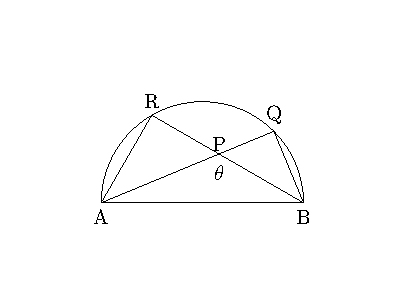
\includegraphics[width=10cm,bb=45 38 149 101]{fig1.pdf}
\end{figure}


\end{document}